\documentclass[elementsmain.tex]{subfiles}
\begin{document}
\section{The Three Viewpoints, Algebraically}

Linear algebra is about solving systems of linear equations. It is also about the geometry of vectors, and it is also about matrices and transformations of one space into another. Somehow, it is all of those things all at the same time, because those are one and the same. Linear algebra is like a gem with many facets, and the beauty of the subject comes out when you learn how to see the light it casts in different directions.

Let's preview the most basic linear algebra situation and three useful geometric ways to look at it.


\subsection*{A Start: the Row Picture}

Consider the following three examples. Each of the first two is a \emph{system of two linear equations in two unknowns}. The third is a \emph{system of three equations in two unknowns}. Because they are familiar, we are using $x$ and $y$ as the names of our unknowns, but we could use other symbols.

\[ \tag{A}\label{eq:A}
\left\{ \begin{array}{rrrrr} 
x & + & 2y & = & 3 \\
 x & + & y & = & 1
\end{array}\right.
\]

\[ \tag{B}\label{eq:B}
\left\{ \begin{array}{rrrrr} 
x & + & 2y & = & 3 \\
3x & + & 6y & = &4
\end{array}\right.
\]

\[ \tag{C}\label{eq:C}
\left\{ \begin{array}{rrrrr}
x & + & 2y & = & 3 \\
 x & + & y & = & 1 \\
3x & + & 6y & = & 4 \\
\end{array}\right.
\]


These are typical examples, though they are ``small.'' In applications, a system of linear equations might have thousands of equations, thousands of unknowns, or both! 

\begin{readingex}
Make a few other examples of systems of linear equations. How are your examples different from those above? How are they the same?
\end{readingex}

Clearly we are looking at equations, so we can ask the kinds of questions that mathematicians always ask when they see equations:
\begin{enumerate}
\item Does the system have any solutions at all? Can we decide before we do a lot of work?
\item If it has solutions, how many solutions are there? Is there a way to tell when the system will have a single unique solution?
\item What is the collection of all solutions? Is there a good way to understand this collection geometrically?
\item Is there a good algorithm for finding solutions? That is, is there an easily-followed-and-not-too-slow computational process for solving the system? Can we make a computer do the work for us?
\item If there is not a solution to the system, can we find an approximate solution? 
Is that a reasonable thing to compute? What should ``approximate solution'' mean in this setting?
\end{enumerate}

Our first goal is to learn to answer these questions for any system of linear equations. 


\begin{readingex}
Can you answer any of the questions in our list for any of the examples above? Or for any of your new examples?
\end{readingex}

Consider how each of these systems is organized by being lined up in rows. 
Each row is a single equation, and that equation defines a collection of points in the $xy$-plane. Since the equation is linear, the collection happens to make a line. (That is why we call them linear equations.) So, we can make a geometric model of each system that involves the interaction of some lines in the $xy$-plane. This geometric model is the \emph{row picture} view of linear algebra. 

Here is the row picture for the system (\ref{eq:A}).
\begin{figure}[h!]
\centering
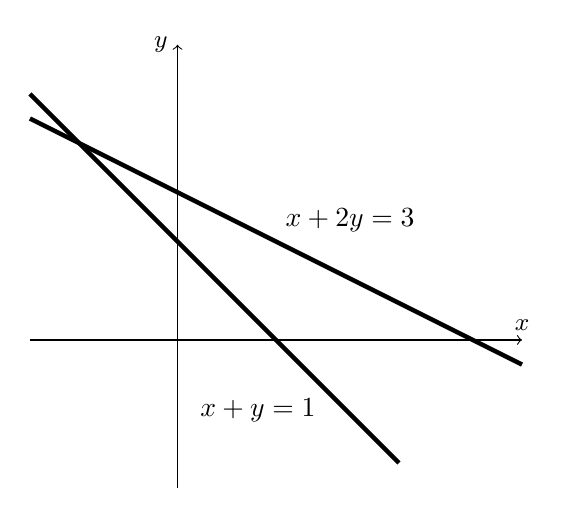
\begin{tikzpicture}[scale=1.25]
\draw[->] (-1.5,0) -- (3.5,0) node[above] {\small $x$};
\draw[->] (0,-1.5) -- (0,3) node[left] {\small $y$};
\draw[ultra thick] (-1.5,9/4) -- (3.5,-1/4);
\node[above right] at (1,1) {$x+2y=3$};
\draw[ultra thick] (-1.5,2.5) -- (9/4,-5/4);
\node[below left] at (1.5,-.5) {$x+y=1$};
\end{tikzpicture}
\caption{The row picture for system (\ref{eq:A})}
\label{fig:rowpic-B}
\end{figure}
In this, we have labeled the two lines with their corresponding equations. The fact that these lines appear to meet gives us a way to talk about the possible solutions to the system (\ref{eq:A}).

\begin{readingex} Make row pictures for the examples you designed above. Can you use these pictures to address any of our questions for your examples?
\end{readingex}

\subsection*{A Second Look: the Column Picture}

Notice that each of our systems is carefully set on the page so that the unknowns line up in columns, too.
We can use that! Let's agree to bundle the coefficients together in columns so that they become objects. Just put each column of coefficients in a set of parentheses. We call these vertical-stacks-of-numbers objects \emph{vectors}, and we reorganize each of our systems into a \emph{linear combination of vectors equation}. The three examples above get reworked to look like this:

\[\tag{A}
x\begin{pmatrix}1\\1\end{pmatrix} + y\begin{pmatrix}2\\1\end{pmatrix} = \begin{pmatrix} 3 \\ 1 \end{pmatrix}
\]

\[\tag{B}
x\begin{pmatrix}1\\3\end{pmatrix} + y\begin{pmatrix}2\\6\end{pmatrix} = \begin{pmatrix} 3 \\ 4 \end{pmatrix}
\]

\[\tag{C}
x\begin{pmatrix}1\\1\\3\end{pmatrix} + y\begin{pmatrix}2\\1\\6\end{pmatrix} = \begin{pmatrix} 3 \\1\\4 \end{pmatrix}
\]


First, we will have to make sense of the algebra of combining vectors like this. This will become the concept of \emph{linear combination}. (We'll come back to the details, soon.) Note that in the first two examples, the vectors all have two entries, but in the third example, the vectors have three entries. These entries are called \emph{coordinates}. Sometimes we talk about the \emph{shape} of a vector, by which we mean the number of coordinates that vector has.

Then we can make a different sort of picture, as \emph{column picture}. Let us do this for system $\ref{eq:B}$. We interpret a vector $\left(\begin{smallmatrix}a \\ b\end{smallmatrix}\right)$ with two components as an arrow which goes from the origin to the point in the plane with Cartesian coordinates $(a,b)$. Drawing all three of the vectors from our situation at once, we have the column picture for system (\ref{eq:B}).
\begin{figure}[h!]
\centering
\begin{tikzpicture}[scale=0.85]
\draw[->] (-1,0) -- (7,0) node[below] {\small $x$};
\draw[->] (0,-1) -- (0,7) node[left] {\small $y$};
\draw[ultra thick,->] (0,0) -- (1,3);
\node[left] at (1,3) {$\begin{pmatrix}1\\3\end{pmatrix}$};
\draw[ultra thick,->] (0,0) -- (2,6);
\node[left] at (2,6) {$\begin{pmatrix}2\\6\end{pmatrix}$};
\draw[ultra thick,->] (0,0) -- (3,4);
\node[right] at (3,4) {$\begin{pmatrix}3\\4\end{pmatrix}$};
\end{tikzpicture}
\caption{The column picture for system (\ref{eq:B})}
\label{fig:colpic-A}
\end{figure}

Notice that the two vectors from the left-hand side of our equation point in the same direction, but the one from the right-hand side points in another direction. This can help us reason about our equation.

\begin{readingex} Translate your examples of systems of equations into the form of a
linear combination equation. Can you also draw their column pictures?
\end{readingex}

Often, a linear combination of vectors equation is written in this compact form
\[
a_1 v_1 + a_2 v_2 + \dots + a_k v_k = w,
\]
where the symbols $a_1, \ldots, a_k$ represent numbers, and the symbols $v_1, \ldots, v_k$ and $w$ represent vectors all having the same shape. This is visually much simpler than the full system.

\subsection*{A Third Look: Matrices and Transformations} 

As we passed from the system of linear equations to the linear combination of vectors equation, we managed to clean up our representation by getting rid of some messy duplication of structural symbols. Now, we will do it again. We take advantage of the  alignment of rows and columns at the same time, and rewrite our equations like this, as \emph{matrix-vector equations}:

\[\tag{A}
\begin{pmatrix} 1 & 2 \\ 1 & 1 \end{pmatrix} \begin{pmatrix}x \\ y \end{pmatrix} 
=\begin{pmatrix}3 \\ 1 \end{pmatrix}
\]

\[\tag{B}
\begin{pmatrix} 1 & 2 \\ 3 & 6 \end{pmatrix} \begin{pmatrix}x \\ y \end{pmatrix} 
=\begin{pmatrix}3 \\ 4 \end{pmatrix}
\]

\[\tag{C}
\begin{pmatrix} 1 & 2 \\ 1 & 1 \\ 3 & 6 \end{pmatrix} \begin{pmatrix}x \\ y \end{pmatrix} 
=\begin{pmatrix}3 \\ 1 \\ 4 \end{pmatrix}
\]


In each case, we have put the two unknowns into a vector, $\left(\begin{smallmatrix} x \\ y \end{smallmatrix}\right)$. The new objects we have introduced are two-dimensional arrays of numbers, called \emph{matrices}. Note that each matrix is constructed by taking the column vectors we found in the linear combination equation and setting them next to each other as columns. The first two examples,
\[
\begin{pmatrix} 2 & 1 \\ 1 & 1 \end{pmatrix} \quad \text{and} \quad \begin{pmatrix} 3 & 1 \\ 51 & 17 \end{pmatrix},
\]
are \emph{$2\times 2$ square matrices} because they have two rows and two columns. The third example, 
\[
\begin{pmatrix}1 & 2 \\ 1 & 1 \\ 3 & 6 \end{pmatrix},
\]
is a \emph{$3 \times 2$ matrix}, because it has three rows and two columns.
In general, the number of rows corresponds to the number of equations, and the number of columns corresponds to the number of unknowns.

\begin{readingex}
Translate your examples into matrix-vector equations.
\end{readingex}


Again, we have to figure out what the algebra of something like ``a matrix times a vector'' should mean, and sort out the geometry of that. The idea is that the matrix represents a kind of \emph{function}, or \emph{transformation}, that takes in vectors of a particular kind, and then gives you back vectors of a (possibly) different kind. In our third example, the matrix takes in vectors like $\left(\begin{smallmatrix} x \\ y \end{smallmatrix}\right)$ with two components, and then gives back vectors with three components.  Since we can represent vectors with two components by arrows in the plane, and vectors with three components by vectors in space, we can make a picture like Figure \ref{fig:trans-pic-C}.

\begin{figure}[h!]
\centering
\begin{tikzpicture}[scale=1.75]
\draw[->] (-5,0) -- (-3,0) node[below right] {\small $x$};
\draw[->, ultra thick] (-4,0) -- (-4.5,.75) node[left] {$x$?};
\draw[->] (-4,-1) node[right] {$\mathbb{R}^2$} -- (-4,1) node[left] {\small $y$};
\draw[->] (-1,0) -- (1,0) node[below] {\small$x_2$};
\draw[<-] (-.75,-.5) node[right] {\small$x_1$} -- (.75,.5) ;
\draw[->, ultra thick] (0,0) -- (.77,.4) node[right] {$b=\begin{pmatrix}3\\1\\4\end{pmatrix}$};
\draw[->] (0,-1) node[right] {$\mathbb{R}^3$} -- (0,1) node[right] {\small $x_3$};
\draw[<-,thick] (-1.25,.25) arc (45:135:1);
\node[below]  at (-2,.25) {$A=\begin{pmatrix}1&2\\1&1\\3&6\end{pmatrix}$};
\end{tikzpicture}
\caption{The transformational view of system (\ref{eq:C})}
\label{fig:trans-pic-C}
\end{figure}



Often, a matrix-vector equation is written in the ultra-compact form
\[
Ax=b,
\] where $A$ is a matrix, $b$ is some known vector, and $x$ is the unknown vector we seek. This form looks simple, because it hides all of the complexity in the abstract matrix and vector objects.


\clearpage

\subsection*{Exercises}

We introduced many concepts and new words in this section, and most of them imprecisely. This should make you feel a bit uneasy, but we will start cleaning up by being more careful in the next section. For now, focus on the shapes and structures of the three (otherwise mysterious) algebraic representations introduced in this section.

\begin{exercise} 
Systems of linear equations come up in all sorts of situations. Here is a typical one. 
When expanded out and rearranged a little, the equation of a circle in the plane takes the form
\[
x^2 + y^2 + ax + by + c = 0.
\]


Suppose that you have a circle which goes through the three points below. Set up the system of linear equations which should help you find the equation of your circle more exactly. (There is no need to solve the system.)
\[
P = (2,3), \qquad Q = (-4,2), \qquad R= (7,1)
\]
How many equations do you have? How many unknowns do you have?

Translate your system of linear equations into a linear combination of vectors equation. What shape to the vectors take? Next, translate your system into a matrix-vector equation of the form $Ax=b$. What shape is the matrix $A$? What shape is the vector $x$? What shape is the vector $b$? 
\end{exercise}

\begin{exercise}
Make an example of a system of two equations in three unknowns. (It's okay. Just pick something you find interesting.) 

Translate your example into a linear combination of vectors equation. What shapes are your vectors? Now translate your system into a matrix-vector equation of the form $Ax=b$. What shape is the matrix $A$? What shape is the vector $x$? What shape is the vector $b$?
\end{exercise}

\begin{exercise}
Make up a matrix-vector equation $Ax=b$ that has a $4\times 2$ matrix. That is, the matrix should have $4$ rows and $2$ columns.

Translate your matrix-vector equation into a linear combination of vectors equation. How many vectors does this have? What shape are they? Then translate your matrix-vector equation into a system of linear equations. How many equations do you have? How many unknowns are there?
\end{exercise}

\begin{exercise}
Make an example of a linear combination of vectors equation that has 5 vectors of the left-hand side of the equal sign, each of which is a stack of 3 numbers.

Translate your equation into a matrix-vector equation. What shape do all of the pieces have? Translate your equation into a system of linear equations. How many equations are there? How many unknowns are there?
\end{exercise}

\begin{exercise}
Think about the ideas discussed in this section. What questions do you have? What do you wonder about?
\end{exercise}

\clearpage
\end{document}








